\section{Protocolli di coerenza}
La coerenza può essere definita formalmente tramite un appropriato invariante, scelto tra:

\begin{itemize}
    \item \textbf{SWMR} (Single Writer Multiple Reader): Durante una data epoca, o c'è un singolo core che può leggere o scrivere la locazione A, oppure un numero di cores che possono solo leggerla.
    \item \textbf{DV} (Data Value): Il valore di A all'inizio di un'epoca è lo stesso valore di A alla fine della sua ultima epoca di lettura/scrittura. 
\end{itemize}

Altre opzioni per i protocolli di coerenza sono operazioni di \textbf{Update}, di fatto transazioni che aggiornano tutte le copie nelle altre cache su una scrittura, o \textbf{Invalidate}, transazioni che invalidano tutte le altre copie su una scrittura. 

\noindent Il protocollo determina la macchina a stati finiti nelle cache e nei controller. Gli inptus alla FSM della cache sono eventi del core (istruzioni di Load/Store, \textit{eviction} di un blocco) e eventi di interconnesione (messaggi \textit{own} e \textit{other's} accettati dall'interconnesione); gli input alla FSM dell'LLC controller sono solo gli eventi di interconnesione. Gli eventi di interconnessione consistono nei messaggi provenienti da altri core diretti al "nostro" core o al memory controller, e nei messaggi \textit{own}: ricevere un messaggio \textit{own} significa che l'interconnesisone ha accettato il messaggio (altrimenti il messaggio risulterebbe \textit{pending} sull'interfaccia di interconnessione). 

\begin{figure}[ht]
    \centering
    \setlength{\fboxrule}{0.5pt} % spessore sottile
    \setlength{\fboxsep}{0pt}    % senza spazio interno
    \fbox{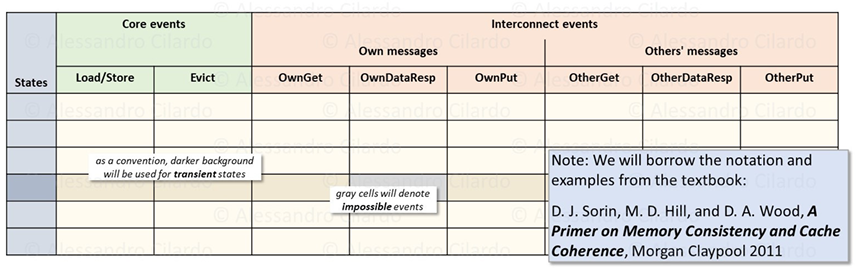
\includegraphics[width=0.8\textwidth]{fig/chapter_3/FSM.png}}
\end{figure}

\begin{warn}
    Una macchina a stati finiti funziona descrivendo un sistema che può trovarsi in un insieme limitato di stati e che cambia stato in base agli ingressi ricevuti. In ogni istante la macchina si trova in uno stato ben preciso, detto stato corrente. Quando riceve un input, consulta le regole di transizione per capire in quale nuovo stato deve andare. A seconda del modello, la macchina può anche produrre un output che dipende solo dallo stato (nel caso di una FSM di Moore) oppure dallo stato e dall'input ricevuto (nel caso di una FSM di Mealy). Questo meccanismo rende le FSM particolarmente utili per descrivere sequenze di eventi o sistemi di controllo.
    Per rappresentarla in una tabella si usa una struttura che mette in relazione gli stati correnti con gli ingressi e specifica quale sarà lo stato successivo e, se previsto, l'output. Una riga della tabella corrisponde a una coppia formata dallo stato corrente e dall'input, mentre le colonne riportano lo stato verso cui si passa e l'eventuale valore di uscita. In questo modo, la tabella diventa una mappa compatta e leggibile che descrive completamente il comportamento della macchina.
\end{warn}

\noindent
Un messaggio di tipo \textbf{Get} rappresenta una \textit{richiesta di lettura o allocazione} di un blocco di memoria. Esso viene tipicamente generato da un core quando si verifica un 
\textit{cache miss}, al fine di occupare una linea della cache con il blocco richiesto. 
L'informazione relativa al tipo di richiesta è codificata nel campo \textit{type} del messaggio. 
Quando un core osserva sull'interconnessione un messaggio di tipo Get emesso da un altro core, esso viene interpretato come \textbf{other Get}. In questo caso, il controller deve verificare se il blocco richiesto è eventualmente presente nella propria cache, per rispondere o per aggiornare lo stato del blocco secondo il protocollo di coerenza adottato.  

\noindent
Il messaggio di tipo \textbf{Put}, invece, è un'operazione di \textit{invio proattivo} di un blocco dalla cache verso il livello inferiore della gerarchia. Ciò avviene tipicamente in caso di \textit{eviction}, ossia quando una linea di cache deve essere liberata. In modo analogo al caso precedente, se un core osserva sull’interconnessione un messaggio di tipo Put proveniente da un altro core, questo viene classificato come \textbf{other Put}.  

\noindent
È importante notare che l'emissione di una richiesta da parte di un cache controller non implica necessariamente la sua immediata accettazione: l'interconnessione può infatti trovarsi in stato \textit{busy}. Per questo motivo, il controller mantiene visibilità delle proprie richieste sotto forma di \textbf{own messages}, che fungono da meccanismo di \textit{acknowledgment} da parte dell'interconnessione, consentendo di sincronizzare la generazione e l'elaborazione dei messaggi.  

\subsection{Protocollo a due stati con Writeback}
In questo protocollo basilare entrambe le FSM hanno due stati, V (Valid) e I (Invalid).
Per le FSM delle cache, V significa che il blocco è disponibile nella cache per lettura/scrittura, mentre I significa che il blocco non è presente in cache. Per l'FSM dell'LLC, V significa che il blocco è in qualche cache di livello superiore, I significa che è disponibile solo nell'LLC. 

\noindent Questo protocollo rispetta gli invarianti di coerenza, ma non supporta molteplici repliche dei dati in nodi diversi quando sono usati solo per operazioni di lettura. 

\begin{warn}
    Lavoriamo sotto l'ipotesi che tutti i messaggi sono inviati in broadcast a tutti i controller e sono visti da tutti nello stesso ordine. Un'ulteriore ipotesi è che gli eventi interni e di interconnesione sono \textit{simultanei} (Load miss $\rightarrow$ OwnGet + DataResp).
\end{warn}

\begin{figure}[ht]
    \centering
    \setlength{\fboxrule}{0.5pt} % spessore sottile
    \setlength{\fboxsep}{0pt}    % senza spazio interno
    \fbox{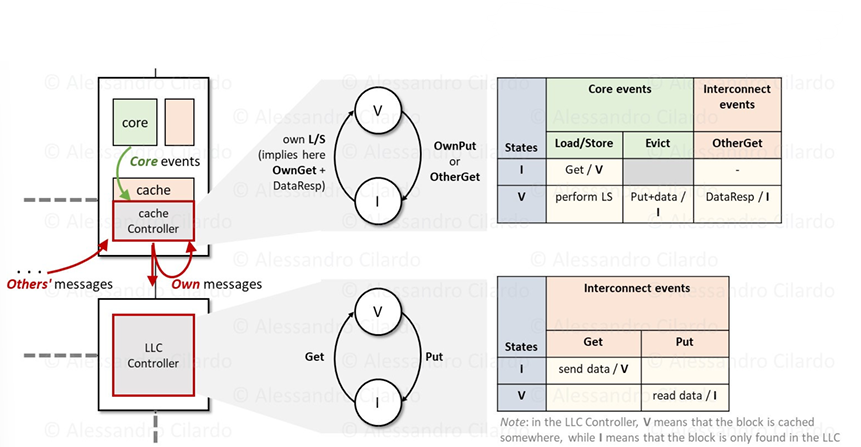
\includegraphics[width=0.85\textwidth]{fig/chapter_3/two_state_protocol.png}}
\end{figure}

\noindent Tipicamente l'interconnessione supporta messaggi di controllo e dato separati, perchè i dati hanno bisogno di risorse di interconnessione (bus) dedicati e impiegano molto più tempo rispetto alle informazioni di controllo. 
Di conseguenza, un interazione di richiesta/risposta deve necessariamente essere gestita da due messaggi separati: Il messaggio di richiesta risposta e il messaggio contenente i dati. \uppercase{è} necessario introdurre degli stati \textit{transienti}, per gestire la situazione in cui un messaggio di controllo è arrivato, ma non sono arrivati i dati. 

\begin{warn}
    Per ora assumiamo che se un core sta aspettando i dati in uno stato transiente, non può intervenire una get proveniente da un altro core. 
\end{warn}

\begin{figure}[ht]
    \centering
    \setlength{\fboxrule}{0.5pt} % spessore sottile
    \setlength{\fboxsep}{0pt}    % senza spazio interno
    \fbox{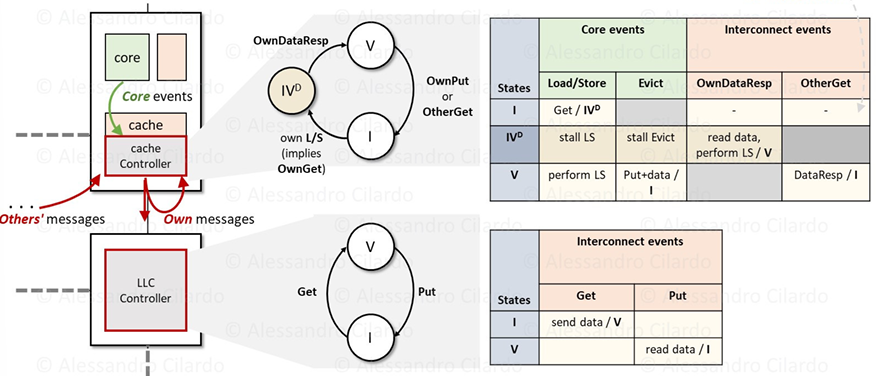
\includegraphics[width=0.85\textwidth]{fig/chapter_3/two_state_protocol_2.png}}
\end{figure}

\subsection{Protocollo a tre stati}